% Probability Two-Dice Markov Process
%
% File:         probability-two-dice-markov-process.tex
% Author:       Bob Walton (walton@acm.org)
% Date:      	Thu Dec 27 01:19:59 EST 2012
  
\documentclass{minimal}
\usepackage[paperheight=2.4in,paperwidth=6in,
            height=2.4in,hoffset=0.05in,
	    voffset=0.05in,left=0in,width=6in]{geometry}
\usepackage{ifthen}
\usepackage{color}
\usepackage[usenames]{xcolor}
\usepackage{scalefnt}
\usepackage{tikz}
\newcommand{\SMALL}{\scalefont{0.8}}
\usetikzlibrary{arrows}
\begin{document}
\raggedright
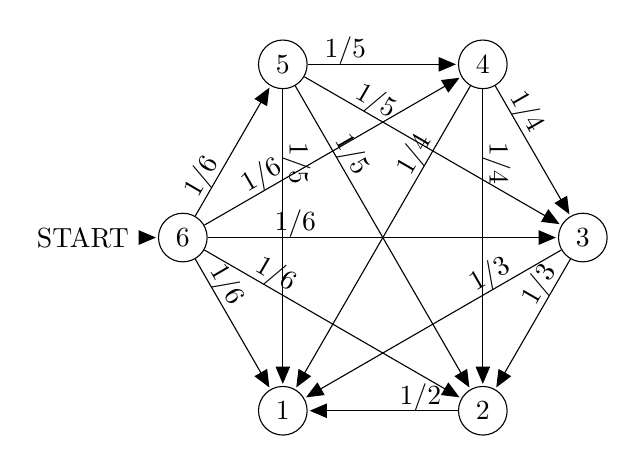
\begin{tikzpicture}[x=1in,y=1in]
\begin{scope}[>=triangle 45,shorten >=0.01in]

    \node (start) at (180:1.5) {START};

    \foreach \n in {1,2,...,6}
    \node[shape=circle,draw] (n\n) at (60*\n+180:1) {\n};

    \draw[->] (start) -- (n6);

    \foreach \n in {2,...,6}
	\foreach \m in {1,2,...,\n}
	{
	    \ifthenelse{\equal{\m}{\n}}
	        {}
		{ \draw[->] (n\n) -- (n\m)
	             node[pos=0.25,sloped,above=-0.05in]{1/\n};
		}
	}
\end{scope}
\end{tikzpicture}
\end{document}
